% can be 9pt
\documentclass[10pt]{sigplanconf}
\usepackage{url}
\usepackage{tikz}
\usepackage{graphicx}
\usepackage{framed}
\usepackage{color}
\usepackage{url}
\usepackage{alltt}
\usepackage{tabularx}
\usepackage{subfigure}
\usepackage{fancyhdr}
\usepackage{paralist}

\usepackage{pgf}

\usepackage{listings}
\lstset{ %
  language=Haskell,                 % the language of the code
  %%basicstyle= \scriptsize,           % the size of the fonts that are used
  %% for the code
  %%firstnumber=0, % index to start numbering at
  %%numbers=left,                      % where to put the line-numbers
  %% numberstyle=\tiny\color{gray},  % the style that is used for the
  %% line-numbers
  %% stepnumber=5,                   % the step between two line-numbers. If it's
                                  % 1, each line
  %%                              % will be numbered
  %% numbersep=5pt,                  % how far the line-numbers are from the code
  %% xleftmargin=0ex,
  %% backgroundcolor=\color{white},      % choose the background color. You must
  %% add \usepackage{color}
  %% showspaces=false,               % show spaces adding particular underscores
  %% showstringspaces=false,         % underline spaces within strings
  %% showtabs=false,                 % show tabs within strings adding
  %% particular underscores
  %% frame=single,                   % adds a frame around the code
  %% rulecolor=\color{black},        % if not set, the frame-color may be
  %% changed on line-breaks within not-black text (e.g. commens (green here))
  %% tabsize=2,                      % sets default tabsize to 2 spaces
  %% captionpos=b,                   % sets the caption-position to bottom
  %% breaklines=true,                % sets automatic line breaking
  %% breakatwhitespace=false,        % sets if automatic breaks should only
  %% happen at whitespace
  %% title=\lstname,                   % show the filename of files included
  %% with \lstinputlisting;
  %%                                 % also try caption instead of title
  %% keywordstyle=\color{blue},          % keyword style
  %% commentstyle=\color{dkgreen},       % comment style
  %% stringstyle=\color{mauve},          % string literal style
  escapeinside={@*}{*@},            % if you want to add a comment within your
                                    % code
  %% morekeywords={*,...}           % if you want to add more keywords to
  %% the set
}


%% \usepackage{tikz}
%% \usetikzlibrary{arrows,automata}

%% \usepackage{amsmath}
%% \usepackage{amsthm}

%% \newtheoremstyle{lst}
%%   {\topsep}   % ABOVESPACE
%%   {\topsep}   % BELOWSPACE
%%   {\itshape}  % BODYFONT
%%   {0pt}       % INDENT (empty value is the same as 0pt)
%%   {} % HEADFONT
%%   {}         % HEADPUNCT
%%   {5pt plus 1pt minus 1pt} % HEADSPACE
%%   {(\thmnumber{#2})}          % CUSTOM-HEAD-SPEC
%% \theoremstyle{lst}
%% \newtheorem{codenum}{lst}

\usepackage{float}
\floatstyle{boxed}
\restylefloat{figure}

%% \include{math}

\newenvironment{code}{\begin{alltt}}{\end{alltt}}
%% \newenvironment{cols}{\begin{tabular}{m{3.6cm}|m{3.6cm}}{Haskell} &

\newcommand{\ttp}[1]{\texttt{#1}}

\usepackage{ifthen}
\newboolean{submission}  %set to true for the submission version
%\setboolean{submission}{false}
\setboolean{submission}{true}
\ifthenelse
{\boolean{submission}}
{ \newcommand{\todo}[1]{ } } %hide todo
{ \newcommand{\todo}[1]{ {\color{blue}$<<$#1$>>$}
 }}
%\usepackage{fancyhdr}

\newcommand{\sub}[1]{\(\sb{#1}\)}

\begin{document}

%% \conferenceinfo{ICFP'12,} {September 9--15, 2012, Copenhagen, Denmark.}
%% \CopyrightYear{2012}
%% \copyrightdata{978-1-4503-1054-3/12/09}

%\titlebanner{banner above paper title}        % These are ignored unless
%\preprintfooter{}   % 'preprint' option specified.

\title{SmartCheck: Automatic and Efficient Counterexample Reduction and Generalization}
%\subtitle{Subtitle Text, if any}

\authorinfo{Lee Pike}
           {Galois, Inc.}
           {leepike@galois.com}
\maketitle

\begin{abstract}
QuickCheck is a powerful library for automatic test-case generation.  Because
QuickCheck performs random testing, it can discover very large counterexamples,
even when enumerating test-cases is infeasible, as is done with SmallCheck.
QuickCheck provides an interface for the user to write a \emph{shrink} function
to attempt to reduce the size of a counterexample discovered by QuickCheck.
Implementations of \emph{shrink} often require significant boilerplate and are
not ``smart'', just generating structurally smaller values.  We introduce
\emph{SmartCheck}, an automatic efficient counterexample reduction algorithm.
SmartCheck reduces algebraic data using generic search heuristics to efficiently
find smaller counterexamples.  In addition to shrinking, SmartCheck generalizes
counterexamples by returning a formula that abstracts over individual
counterexamples.  SmartCheck has been implemented for Haskell and tested on a
variety of Haskell programs.
\end{abstract}

%% \category{D.2.4}{Software/Program Verification}{Reliability}

%% \terms
%% Languages, Verification

%% \keywords
%% embedded domain-specific language, compiler, verification

\todo{define variant, tag}
\todo{note constants are user-defined arguments, other simplifications}

\section{Introduction}\label{sec:intro}
The QuickCheck testing framework was a revolutionary step-forward in
type-directed random testing~\cite{qc}.  Originally designed for Haskell,
QuickCheck has been ported to other languages and is a now a widely-used testing
tool.  Because QuickCheck generates random values for testing, counterexamples
it finds may be substantially larger than a minimal counterexample.  In their
original QuickCheck paper~\cite{qc}, the authors report the following user
experience by Andy Gill:
%
\begin{quote}
Sometimes the counterexamples found are very large and it is difficult to go
back to the property and understand why it is a counterexample.
\end{quote}
%
\noindent
QuickCheck defines a type class \ttp{Arbitrary} that presents a method
\ttp{arbitrary} for generating random values of a given type.  Gill added another
method to the type class:
%
\begin{code}
smaller :: a -> [a]
\end{code}
%
\noindent
The purpose of \ttp{smaller} is to generate strictly smaller values (according to
some measure) from a given counterexample to attempt to find a smaller
counterexample.  Today, \ttp{smaller} is called \ttp{shrink}.

\begin{figure}[ht]
\begin{code}
data A = A Int16 deriving Show

data B = B [A] [A] [A] [A] deriving Show

-- QuickCheck instances
instance Arbitrary A where
  arbitrary    = liftM A arbitrary
  shrink (A i) = map A (shrink i)

instance Arbitrary B where
  arbitrary = liftM4 B arbitrary arbitrary
                       arbitrary arbitrary
  shrink (B a b c d) =
    [ B w x y z | w <- shrink a
                , x <- shrink b
                , y <- shrink c
                , z <- shrink d ]

-- SmallCheck instances
instance Serial Int16 where
  series d = drawnFrom [(-d')..d']
    where d' = fromIntegral d

instance Serial A where series = cons1 A
instance Serial B where series = cons4 B

-- Predicates for defining properties
add :: [A] -> Int16
add = sum . map (\(\backslash\)(A i) -> i)

pre :: B -> Bool
pre (B a b c d) =
  all (\(\backslash\) -> add x < 16) [a, b, c, d]

post :: B -> Bool
post (B a b c d) =
  add a + add b + add c + add d < 64

-- Property
prop :: B -> Property
prop p = pre p ==> post p
\end{code}
  \caption{QuickCheck and SmallCheck for a product-type input.}
  \label{fig:initial}
\end{figure}

While \ttp{shrink} is user-defined and can have any type-correct implementation,
it is typically defined using structural recursion for composite data types.
For example, consider the \ttp{shrink} instances given to data types \ttp{A} and
\ttp{B} in Figure~\ref{fig:initial}.\footnote{All examples and algorithms in
  this paper are presented in Haskell~\cite{haskell98}.}  Indeed, because of the regular
structure of \ttp{shrink} implementations, the principal motivation for one of
Haskell's first generics package was for providing generic definitions for
\ttp{shrink}~\cite{syb}.

However, this straightforward approach to defining \ttp{shrink} instances may
either miss minimal counterexamples, be too inefficient to be practical, or
both.\footnote{For a recent real-world case, see the user question posed on
  StackOverflow:
  \url{http://stackoverflow.com/questions/8788542/how-do-i-get-good-small-shrinks-out-of-quickcheck}.}
For example, consider again Figure~\ref{fig:initial}.  The data type \ttp{B} is
a product type over lists of 16-bit signed integers, wrapped by a constructor.
Consider the property \ttp{prop} in the figure, stating that if the sum of each
list in a field of \ttp{B} is less than 16, then the sum of the four fields is
less than 64.  The property \ttp{prop} seems reasonable at first glance, until
one realizes that due to underflow, the property can be violated.  For example,
consider the value
%
\begin{code}
B [A (-32769)] [] [] []
\end{code}
%
\noindent
Without shrinking, QuickCheck finds large examples to the property; on average,
QuickCheck returns a value contains 70 \ttp{Int16} values!

Thus, it pays to define \ttp{shrink}.  Unfortunately, even for a simple property
and program like this one, the definition for \ttp{shrink} given in
Figure~\ref{fig:initial} produces an intractable number of potential
counterexamples to test; with the definitions and property provided (together
with QuickCheck's default \ttp{Arbitrary} instance for lists), the list of
potential counterexamples generated by \ttp{shrink} can contain more than
$10^{10}$ elements.  This is an enormous state space to search for a smaller
example and can cause the shrinking phase to take orders-of-magnitude more time
than the counterexample discovery phase.

It is not always straightforward to determine how to make a more efficient
implementation for \ttp{shrink}.  Shrinking presents a programmer's dilemma:
shrinking is used to better understand a counterexample to understand why a
property failed, but to implement an efficient shrink function in general
requires knowing how to generate counterexamples to the property.

Typically, a user tries a brute-force approach to reduce the number of potential
counterexamples, for example, by truncating lists using the (\ttp{take n}) function
that returns the first $n$ elements of a list.  The trade-off is quicker
shrinking with a lower probability of finding a smaller counterexample.  For
example, redefining shrink for type \ttp{B} as follows
%

%% \begin{minipage}{\columnwidth}
%% \lstset{ caption={Truncated shrinking function for data type \ttp{B}.}
%%        , label=lst:newshrink
%%        , captionpos=b }
%% \begin{lstlisting}

\begin{figure}[ht]
\begin{code}
len = 10

shrink (B a b c d) =
  [ B w x y z | w <- tk a, x <- tk b
              , y <- tk c, z <- tk d ]
  where tk x = take len (shrink x)
\end{code}
  \caption{Truncated shrinking function for data type \ttp{B}.}
  \label{lst:newshrink}
\end{figure}

%% \end{lstlisting}
%% \end{minipage}
%
\noindent
controls the exponential blowup of the state-space by taking the first ten
elements of each list, so the cross product is limited to 1000 elements.  The
downside is that potentially smaller counterexamples may be omitted.

The programmer might ask herself: ``What if we omit the need for shrinking
counterexamples altogether?''  SmallCheck is another testing framework for
Haskell that does just this.  SmallCheck is guaranteed to return the a smallest
counterexample, if one exists~\cite{sc}.  SmallCheck does this by enumerating
all possible inputs, ordered from smallest to largest, up to some user-defined
bound.  While SmallCheck is effective for testing many programs and properties
(in accordance with the \emph{small scope hypothesis}~\cite{jackson}),
counterexamples to even relatively simple properties may be infeasible to
discover due to state-space explosion.

With SmallCheck, a property is checked up to a depth set by the user, measuring
how large values are.  For example, for type \ttp{Int}, the depth $d$ is defined
as the integers in the list enumerating from $-d$ to $d$ (i.e.,
\ttp{[(-d)..d]}).  For a product type, SmallCheck must check values produced by
taking the cross-product of the type's fields at a given depth.  In
Figure~\ref{fig:initial}, we have defined instances for generating Lazy
SmallCheck (a variant of SmallCheck) tests by defining instances
for the \ttp{Serial} class.  For the property \ttp{prop} defined above (suitably
redefined to use SmallCheck's types), SmallCheck must check to depth 16 to find
the first counterexample.  Unfortunately, after a couple hours of testing, Lazy
SmallCheck is still checking values at depth six, and the number of tests scales
exponentially with respect to the depth.\footnote{All tests in this paper are
  performed on a four-core Pentium~i7 running at 2.7GHz with 8GB RAM on
  Fedora~16.  This test, and others unless noted, are performed using
  interpreted Haskell under GHC 7.4.2.}

Finally, even if we could overcome the problems described above with QuickCheck
and SmallCheck, we are left with two others.
\begin{itemize}
  \item First, when a counterexample is discovered to some property, say with
    type
%
\begin{code}
prop :: B -> Bool
\end{code}
%
\noindent
one might wish to search for different counterexamples to \ttp{prop}.  Ideally,
the testing framework would automatically add a predicate characterizing (and
perhaps generalizing) a counterexample
%
\begin{code}
cex :: B -> Bool
\end{code}
%
\noindent
as a precondition to \ttp{prop} to define a new property
\begin{code}
prop' b = not (cex b) ==> prop b
\end{code}
%
\noindent
where \ttp{==>} is implication to generate new counterexamples to the same property.

  \item Second, and more generally, a counterexample is usually representative
    of other counterexamples, but that generalization is left to the user to
    discover for herself.  Really, what would be useful would be not just a
    minimal counterexample, but a quantified formula characterizing a set of
    counterexamples.  Such a formula has the added benefit of replacing a
    potentially large sub-term of a composite data type value with a quantifier.
\end{itemize}

\begin{table}[ht]
\footnotesize
  \begin{center}
    \begin{tabular}{|r||c|c|c|c|}
\hline
 & QC (none) & QC (10) & QC (20) & SmartCheck \\
\hline \hline
Max.  & 0.15s & 21.51s & 125.37s & 1.96s\\
\hline
Mean  & 0.07s & 1.21s & 3.80s & 0.30s\\
\hline
Median & 0.07s & 0.48s & 0.52s & 0.24s\\
\hline
Mean size & 70 & 34 & 32 & 5\\
\hline
    \end{tabular}
  \end{center}
  \caption{Results for 100 tests of the program in Figure~\ref{fig:initial}
    using interpreted Haskell.}
  \label{table:results}
\end{table}


\paragraph{SmartCheck}
Motivated by these limitations of QuickCheck and SmallCheck, we have developed
\emph{SmartCheck}.  SmartCheck extends QuickCheck to efficiently and generically
find small counterexamples as well as generalize them as described in the
preceding paragraph.  To motivate the benefit of SmartCheck, consider the table
in Table~\ref{table:results}, giving the results for using QuickCheck and
SmartCheck on the program shown in Figure~\ref{fig:initial} (we omit SmallCheck,
since as we noted, it is not even feasible for an example like this).  In the
first three columns, the results of using QuickCheck to generate counterexamples
are shown.  The first column contains the results of using QuickCheck without
shrinking to provide a baseline.  The next two columns show the result of using
QuickCheck with definitions of \ttp{shrink} that limit the lists of fields of
\ttp{B} to 10 (Figure~\ref{lst:newshrink}) and 20 elements
(Figure~\ref{lst:newshrink}, with \ttp{len = 20}), respectively.  (Recall that
with the original definition for shrink from Figure~\ref{fig:initial}, some
counterexamples cause QuickCheck to not return after hours of computation.)  In
each row, we show the maximum, mean, and median number of seconds required by
QuickCheck to generate a counterexample over 100 runs.  In the last row, we show
the mean size of the final value returned, measured by the taking the cumulative
length of the lists of the fields of \ttp{B}.  Notice that while typically
counterexamples are returned in a fraction of a second, there are outliers
taking 21 seconds and 125 seconds for the two tests.  Both tests roughly cut the
size of the counterexample in half; increasing the number of potential
counterexamples can result in a significant performance penalty for this example
without much benefit.

In the last column are the results for SmartCheck.  Not only does it execute
faster than QuickCheck with shrinking, it has significantly smaller outliers.
The most striking difference, however, is the size of the counterexample
returned, reducing on average the size of a counterexample found by QuickCheck
without shrinking by a factor of 14.

The purpose of this paper is to explain first how to efficiently and generically
generate small counterexamples for algebraic data types and second how to
generalize the counterexamples.

\todo{check paper against this section again, especially generalization sec.}
\paragraph{Contributions}
This paper, and the library it describes, makes the following contributions:

\begin{itemize}

\item an efficient counterexample reduction strategy for algebraic
  data types;

\item an approach to counterexample generalization, to present the
  user with a formula describing a set of counterexamples to a property;

\item an approach to generically strengthen a property with a precondition that
  characterizes an already-discovered counterexample for the purpose of finding
  new, dissimilar counterexamples;

\item an implementation based on generic programming that is not only more
  efficient that hand-written \ttp{shrink} instances in many cases but that
  generates the instances automatically for the user.

%% \item More generally, this paper is the first to explore the idea of
%%   efficient, generic counterexample reduction and generalization for
%%   functional program testing.
\end{itemize}

%% \noindent Moreover, the inability to quickly uncover understandable
%% counterexamples is a real-world problem with QuickCheck (or other functional
%% languages).  It works great when your tests pass,

\paragraph{Outline.}
The paper precedes as follows.  We define a type class and some definitions in
Section~\ref{sec:preliminaries} used in the remainder of the paper.  In
Section~\ref{sec:shrinking}, we describe SmartCheck's reduction algorithm for
efficiently shrinking large counterexamples.  In
Section~\ref{sec:generalization}, we turn our attention to the problem of
counterexample generalization.  Here, we present two algorithms for generalizing
counterexamples and constructing formulas for describing them.  We also discuss
a method for property strengthening to discover new counterexamples.  We
describe implementation-specific details in Section~\ref{sec:implementation},
and the results of some experiments in using our tool are presented in
Section~\ref{sec:experiments}.  Related work is given in
Section~\ref{sec:related}.  Finally, concluding remarks and future work are
presented in Section~\ref{sec:conclusions}.


%%%%%%%%%%%%%%%%%%%%%%%%%%%%%%%%%%%%%%%%%%%%%%%%
\section{Preliminaries}\label{sec:preliminaries}

To present the algorithms in the following sections, we provide some definitions
here.  Our presentation simplifies the implementation
(Section~\ref{sec:implementation}) somewhat to improve the presentation.
Consider the following types and type class.
%
\begin{code}
type Idx    = Int
type Size   = Int
data SubVal = forall a. SubTypes a => SubVal a

class Arbitrary a => SubTypes a where
  size    :: a -> Size
  index   :: a -> Idx -> Maybe SubVal
  replace :: a -> Idx -> SubVal -> a
  constr  :: a -> String
  constrs :: a -> [String]
\end{code}
%
\noindent
The \ttp{SubTypes} type class requires QuickCheck's \ttp{Arbitrary} as a
super-class.  \ttp{SubTypes} has five methods.  The \ttp{size} method returns
the size of a value, \ttp{index} returns a sub-value at an breadth-first index
in a value, \ttp{replace} replaces a sub-value at a particular focus,
\ttp{constr} returns the constructor tagging the value, and \ttp{constrs}
returns a list of unique identifiers for the constructors associated with each
variant of the type.

For example, consider a binary tree type:
%
\begin{code}
data Tree = L | B Tree Tree
\end{code}
%
\noindent
and the value \ttp{tree}, labeled with the indexes of its sub-values
%
\begin{code}
tree = B\sub{0} (B\sub{1} L\sub{3}
             (B\sub{4} L\sub{6} L\sub{8}))
          (B\sub{2} L\sub{5} L\sub{7})
\end{code}
%
\noindent
Here are example applications of \ttp{SubTypes} methods; in the following, we
show the indexes with respect to the \ttp{tree} value:
%
\begin{code}
size tree = 9

index tree 4  = (Just . SubVal) (B\sub{4} L\sub{6} L\sub{8})
index tree 12 = Nothing

replace tree 2 (SubVal L) =
  B\sub{0} (B\sub{1} L\sub{3}
        (B\sub{4} L\sub{6} L\sub{8}))
     L

constr  tree = ["B"]
constrs tree = ["B", "L"]
constrs L    = ["B", "L"]
\end{code}
%
\noindent
We will sometimes refer to the unwrapped value returned by \ttp{index a i} as
the \emph{$i$th sub-value of $a$}, so for example, \ttp{B\sub{4} L\sub{6}
  L\sub{8}} is the 4th sub-value of \ttp{tree}.  An invariant of \ttp{index} is
that for any value \ttp{a}, consider the least $i \geq 0$ such that $$\ttp{index
  a i} = \ttp{Nothing}$$ For all $0 \leq j < i$, $$\ttp{index a j} \neq
\ttp{Nothing}$$ We use this invariant as a termination case in recursive
algorithms over the sub-values of a value.

The method \ttp{replace} returns the original value for an out-of-bounds index
or an incorrectly-typed replacement value.  The \ttp{SubVal} type is an
existential data type, used as a generic container for sub-values from a
counterexample.

Finally, while \ttp{constr} returns a string representation of the constructor
associated with the specific variant passed to it, \ttp{constrs} ignores the
value and returns the same list of constructors for any value from the type.
(In our implementation, \ttp{constrs} depends on GHC Generics~\cite{generics},
which we describe in Section~\ref{sec:implementation}.  For simplicity, we omit
here Generics-specific super-class constraints on the \ttp{SubTypes} class.)

% ------------------------------------------------------------------------------

\section{Shrinking Data}\label{sec:shrinking}
In this section, we describe how to efficiently shrink data values.  Before we
begin, recall the basic idea behind the \ttp{shrink} method of the
\ttp{Arbitrary} class: generate a list of values, each of which is smaller than
the current counterexample.  Each of the new values generated typically bears no
relationship to the original counterexample other than being smaller.

Consider the problem of finding a small counterexample as a graph search
problem.  The set of vertexes are all possible well-typed values.  There is an
edge from vertex $v$ to $v'$ if $v'$ is smaller than $v$ by some measure.  The
goal is to traverse the graph, starting from a counterexample, to find a vertex
from the set of smallest counterexamples in the graph.

The approach taken by \ttp{shrink} is the most naive graph search algorithm: it
simply generates a random set of potential vertexes to check in the graph.
However, it does not exploit that the original counterexample \ttp{cex} is
already in a neighborhood of other likely counterexamples.  So rather than
choose random vertexes, it may be more efficient to test other values that are
closely related to \ttp{cex}.  By restricting the search to \ttp{cex}'s
neighborhood, a smaller counterexample might be missed, and only a local minimum
is returned.  However, with a large state space, finding a global minimum by
random sampling vertexes in the graph is possible but too inefficient, as we saw
from the example in the introduction.

\subsection{Reduction Algorithm Overview}\label{sec:reduct}
The algorithm we present for efficiently searching for new counterexamples can
be thought of as a recursive breadth-first traversal over the structure of the
current counterexample value, where the value is represented as a tree.  At each
node, during the traversal, we generate arbitrary \emph{structurally} smaller
sub-values and build a new value from that, leaving the remainder of the tree
unchanged.  Intuitively, by a structurally smaller value, we mean one with fewer
constructors.  We continue until we reach a fixed-point.


\begin{figure}[ht]
  \lstset{caption={}
%         ,xleftmargin=5ex,firstnumber=0,numbers=left
         }
  \begin{code}
getSize :: SubVal -> Size
getSize (SubVal a) = size a

newVals :: SubVal -> Size -> Int -> IO [SubVal]
newVals (SubVal a) sz tries =
  replicateM tries s
  where
  s  = liftM SubVal (sizedArbitrary sz a)

reduce :: SubTypes a
       => a -> (a -> Property) -> IO a
reduce cex prop = reduce' 1
  where
  reduce' idx =
    case index cex idx of
      Nothing -> return cex
      Just v  -> do
        vs <- newVals v (getSize v) scMaxReduce
        case test cex idx vs prop of
          Nothing   -> reduce' (idx+1)
          Just cex' -> reduce cex' prop

test :: SubTypes a => a -> Idx -> [SubVal]
     -> (a -> Property) -> Maybe a
test cex idx vs prop = go vs
  where
  go []      = Nothing
  go (v:vs') =
    let cex' = replace cex idx v in
    if pass prop cex' then go vs'
      else Just cex'
  \end{code}
  \caption{Counterexample reduction algorithm.\label{fig:reduction}}
\end{figure}

Figure~\ref{fig:reduction} shows the reduction algorithm.  The function
\ttp{reduce} takes a counterexample \ttp{cex} and the property \ttp{prop}.  At
the beginning of execution, we assume that a counterexample has been obtained
somehow; our implementation relies on QuickCheck as a ``front-end'' to generate
a counterexample that the algorithm automatically shrinks.  The reduction begins
at the first sub-value of \ttp{cex}, \ttp{v}.  When the index \ttp{idx} becomes
out-of-bounds and returns \ttp{Nothing}, the algorithm terminates.  Otherwise, a
list of new random values are generated.
%
\begin{code}
sizedArbitrary :: SubTypes a => a -> IO a
\end{code}
%
\noindent
generates a new value \ttp{v'} having the same type as \ttp{v} and strictly
smaller (with respect to the \ttp{size} method) than \ttp{v}.  Just like
QuickCheck's \ttp{arbitrary} method, \ttp{sizedArbitrary} generates successfully
larger counterexamples when generating new values with which to replace a
sub-value.

\todo{explain getSize}

\ttp{sizedArbitrary} returns a value inside the \ttp{IO} monad since it depends
on a random seed for generation (we could pass in the generator seed, but for
simplicity, we assume one is generated locally).  The constant \ttp{scMaxReduce} is
the maximum number of tries to discover a new counterexample by replacing
\ttp{v} in \ttp{cex} and testing it.  The result of \ttp{pass prop cex'} for
%
\begin{code}
pass :: (a -> Property) -> a -> Bool
\end{code}
%
\noindent
holds if \ttp{cex'} satisfies the property \ttp{prop}.  If no failure is found,
we move to the next sub-value of \ttp{cex} and continue.  However, if a new
smaller counterexample \ttp{cex'} is found, we start a new breadth-first
traversal of \ttp{cex'}, attempting to shrink it further.

\subsection{Reduction Algorithm Details and Optimizations}
The reduction algorithm description above omits some minor details and
optimizations we describe here.

\subsubsection{Sum-type counterexample hypothesis}
First, recall that the algorithm begins at the \emph{first} sub-value of the
counterexample rather than the 0th sub-value.  The 0th sub-value of \ttp{cex} is
\ttp{cex} itself.  No invariant of the algorithm would be violated by beginning
with the 0th sub-value; recall that it would generate strictly smaller values
than \ttp{cex}.  However, we begin with a strict sub-value because of a
hypothesis we refer to as the \emph{sum-type counterexample hypothesis}.  The
hypothesis is that in the search space of possible values, if a counterexample
of the form \ttp{C}~$\vec{x}$, where \ttp{C} is some constructor and $\vec{x}$
are its arguments, is discovered, then it is more likely to find another
``nearby'' counterexample of the form \ttp{C}~$\vec{y}$, where $\vec{y}$ are
different arguments to \ttp{C}.  For example, consider a property about
unintended variable capture over a language's parse tree represented by a sum
type with constructors for module imports, function definitions, and
global-variable assignments, respectively.  A function definition counterexample
can only be reduced to smaller function definition counterexamples, the only
construct in which variable capture is possible.

Another way to motivate the hypothesis is that searching the space of possible
counterexamples by generating \emph{any} well-typed value that is strictly
smaller than the original counterexample is something we have seen before: it is
precisely the naive approach to implementing \ttp{shrink}!

\subsubsection{Conditional properties}
A QuickCheck property may be a conditional of the form
%
\begin{code}
prop a = pre a ==> prop' a
\end{code}
%
\noindent
such that \ttp{prop} is true if the precondition \ttp{pre a} is false or
\ttp{prop' a} holds.  In practice, conditionals are used to restrict the set of
values tested; values that fail the precondition are discarded.  Thus, the call
to \ttp{pass} in the reduction algorithm only considers a potential
counterexample \ttp{cex} to have failed if it passes the property's
precondition and fails the consequent.

\subsubsection{Sub-value counterexample hypothesis}\label{sec:subval}
Sometimes, a counterexample fails a property due to a sub-value nested deep
inside the counterexample.  The rest of the value is irrelevant.  We call this
the \emph{sub-value counterexample hypothesis.}  Thus, one way to efficiently
search the space of potential counterexamples is to test a counterexample's
(well-typed) sub-values.

For example, consider a simple calculator language containing constant
\ttp{Ints}, addition, and division:
%
\begin{code}
data Exp = C Int
         | Add Exp Exp
         | Div Exp Exp
\end{code}
%
\noindent
and consider an interpreter for the language that returns \ttp{Nothing} if
division-by-zero is encountered and \ttp{Just} the value otherwise:
%
\begin{code}
eval :: Exp -> Maybe Int
eval (C i) = Just i
eval (Add e0 e1) =
  liftM2 (+) (eval e0) (eval e1)
eval (Div e0 e1) =
  let e = eval e1 in
  if e == Just 0 then Nothing
    else liftM2 div (eval e0) e
\end{code}
%
\noindent
Suppose we restrict the set of programs with the following predicate:
%
\begin{code}
divSubTerms :: Exp -> Bool
divSubTerms (C _)         = True
divSubTerms (Div _ (C 0)) = False
divSubTerms (Add e0 e1)   =    divSubTerms e0
                            && divSubTerms e1
divSubTerms (Div e0 e1)   =    divSubTerms e0
                            && divSubTerms e1
\end{code}
%
and then test the property
%
\begin{code}
prop_div e = divSubTerms e ==> eval e /= Nothing
\end{code}
%
\noindent
The property \ttp{prop\_div} turns out to be false; for example,
%
\begin{code}
Div (C 1) (Div (C 0) (C 1))
\end{code}
%
\noindent
is a counterexample.  In the predicate case
%
\begin{code}
divSubTerms (Div _ (C 0)) = False
\end{code}
%
\noindent
we forgot to recur on the divisor.

\begin{figure}[ht!]
\ttp{Div (Div (C (-22)) (Div (C 2) (C 13))) (Div (Div (Div (C (-11)) (C 14))
  (Add (Div (C (-4)) (C (-3))) (Div (C (-25)) (C (-25))))) (Add (Add (C 22) (Div
  (C (-30)) (C (-14)))) (C 13)))}
  \caption{Typical counterexample from QuickCheck with no user-defined
    \ttp{shrink} function.}
  \label{fig:div-cex}
\end{figure}

However, a typical counterexample returned by QuickCheck, without \ttp{shrink}
implemented, is shown in Figure~\ref{fig:div-cex}.  To butcher an expression,
finding the cause of failure is like searching for a divide-by-zero in the
haystack!  But it turns out that the culprit is a small sub-value:
%
\begin{code}
Div (C (-22)) (Div (C 2) (C 13))
\end{code}
%

\begin{figure}
\begin{code}
reduce0 :: forall a . SubTypes a
        => a -> (a -> Property) -> IO a
reduce0 cex prop = reduce' 1
  where
  reduce' idx =
    case index cex idx of
      Nothing -> return cex
      Just v  -> case testHole v of
                   Just v' -> reduce0 v' prop
                   Nothing -> test' v idx

  test' v idx = do
    vs <- newVals v (getSize v) scMaxReduce
    case test cex idx vs prop of
      Nothing   -> reduce' (idx+1)
      Just cex' -> reduce0 cex' prop

  testHole (SubVal a) =
    case cast a :: Maybe a of
      Nothing -> Nothing
      Just a' ->
        if pass prop a' then Nothing
          else Just a'
\end{code}
  \caption{Reduction algorithm with the sub-value counterexample optimization.}
  \label{fig:reduce0}
\end{figure}

Generalizing this scenario, during the reduction algorithm's breadth-first
search through a counterexample \ttp{cex}'s sub-values, we may happen upon a
sub-value \ttp{cex'} that has the same type as \ttp{cex} and fails the property
(while passing any preconditions).  In this case, we can return \ttp{cex'}
directly, and rerun the reduction algorithm on \ttp{cex'}.  In
Figure~\ref{fig:reduce0}, we show an updated reduction algorithm, \ttp{reduce0}
that implements this optimization.  The function \ttp{testHole} tests the
current sub-value and if it fails the property, the function tests the sub-value
directly.

\subsubsection{Base types}

The number of constructors in an algebraic data value primarily determines how
large and understandable it is.  In our experience, the size of fields that come
from primitive types, like \ttp{Int} or \ttp{Char}, have less of a role in
understanding a counterexample.

Consequently, we distinguish a class of types referred to as \emph{base types}.
If the reduction algorithm encounters a base type, it is ignored.  By default,
this includes numeric types (e.g., \ttp{Int}, \ttp{Word}, \ttp{Float}, etc.,
\ttp{Bool}, and \ttp{Char}.  We also treat lists specially: lists of base types
are considered to be base types themselves.  This prevents the algorithm from
analyzing, for example, strings.  A list of a non-base-types is shrunk by the
algorithm.

By providing custom instances, the user can declare any substructure in a data
type to be a base type.  Doing so can help make SmartCheck more efficient if the
user knows that some portion of the structure cannot be shrunk or is irrelevant
to the property.

\subsubsection{Bounding counterexample exploration}

SmartCheck's implementation contains flags to allow the user to customize its
behavior.  Three flags that are relevant to the reduction algorithm are the
following:
%
\begin{code}
scMaxReduce :: Int
scMaxSize   :: Int
scMaxDepth  :: Maybe Int
\end{code}
%
\noindent
The \ttp{scMaxReduce} flag controls the number of values generated by the
reduction algorithm for each sub-value analyzed.  \ttp{scMaxSize} controls the
maximum size of values generated to replace sub-values by the reduction
algorithm.  Thus, new sub-values must be strictly smaller than the minimum of
\ttp{scMaxSize} and the size of the sub-value being replaced.  (The size of the
value is with respect to the \ttp{size} method in the \ttp{SubTypes} class.)
Finally, \ttp{scMaxDepth} determines the maximum depth in the counterexample the
reduction algorithm should analyze.  A value of \ttp{Nothing} means that the
counterexample should be exhaustively reduced, as the algorithm is presented in
Figure~\ref{fig:reduction}.  For example, the depth of a list is determined by
its length and the depth of the binary tree defined in Section~\ref{sec:reduct}
is determined by the function \ttp{depth}:
%
\begin{code}
depth L         = 0
depth (B t0 t1) =
  1 + max (depth t0) (depth t1)
\end{code}
%
\noindent
Of the flags, \ttp{scMaxDepth} is the most important for controlling
efficiency, particularly for large product types with significant ``fan out''.
The number of sub-values of a value product type can grow exponentially with
respect to the depth.  Furthermore, note that as the reduction algorithm
descends further, there is less chance to reduce the size of the value overall,
since smaller and smaller sub-values are replaced.

\section{Counterexample Generalization}\label{sec:generalization}

Small counterexamples make debugging easier, but they are just half the battle.
To go from a specific counterexample to the required fix in a program, the
programmer must have a flash of insight in which she generalizes the
counterexample to a set of counterexamples for which the program and property
fails.  For example, in the introduction, we realized that the specific
counterexample
%
\begin{code}
B [A (-32769)] [] [] []
\end{code}
%
\noindent
is representative of the set of counterexamples in which underflow causes the
sum of the fields to be greater or equal to 64.

The generalization step is an important under-appreciated step in the debugging
process.  For counterexamples that are large, deeply-nested values, the
generalization step can be difficult.  One way we might help the programmer is
to provide her not with a single counterexample but with a quantified formula
that characterizes a set of counterexamples.  Doing so has two benefits.  First,
it already generalizes a counterexample, perhaps helping the programmer's
insight in the generalization step.  Second, it reduces the noise in favor of
the signal by abstracting away portions of large counterexample that are
irrelevant to why it violates the property.

The characterization of counterexamples that most helps the programmer seems to
should strike a middle ground.  At the one extreme, a single counterexample is
can be thought of as a closed formula containing only literals that
under-approximates the set of counterexamples.  At the other extreme, the
property itself being tested is a formula that over-approximates the failing
inputs.  We describe two kinds of formula that fall between these two extremes.

\subsection{Universal Sub-Value Generalization}\label{sec:universal}
An example best explains the first kind of quantified formulas we generate.
Compare the following formula to the counterexample in Figure~\ref{fig:div-cex}:
%
\begin{code}
\ttp{forall x, y . Div (Div x (Div (C 2) (C 13))) y}
\end{code}
%
\noindent
Here, the formula claims that for all well-typed values \ttp{x} and \ttp{y}, the
property fails.  Not only does the generalization assist the programmer's
insight, but it reduces the sheer size of the counterexample, and it can do so
significantly.  We call the kind of formula just shown \emph{universal sub-value
  generalization} and is implemented in SmartCheck.

An extrapolation algorithm performs universal sub-value generalization.  The
basic idea is as follows: for a counterexample \ttp{cex} and a property
\ttp{prop}, a breadth-first search over the sub-values of the \ttp{cex} is
performed.  For each sub-value, the algorithm generates new sub-values, replaces
them in \ttp{cex} to create a list of new potential counterexamples.  If enough
new counterexamples non-trivially fails \ttp{prop} (i.e., does not just fail the
precondition), and non satisfy \ttp{prop}, then we extrapolate, claiming that
for \emph{any} new value replacing that sub-value in \ttp{cex}, the property
will fail.

\begin{figure}
  \begin{code}
subTrees :: SubTypes a => a -> Idx -> [Idx] -> Bool
subTrees cex idx = any (subTree cex idx)

extrapolate :: SubTypes a
            => a -> (a -> Property) -> IO [Idx]
extrapolate cex prop = extrapolate' 1 []
  where
  extrapolate' idx idxs
    | subTrees cex idx idxs
    = extrapolate' (idx+1) idxs
    | otherwise
    = case index cex idx of
        Nothing -> return idxs
        Just v  -> do
          vs <- newVals v scMaxSize scMaxExtrap
          extrapolate' (idx+1)
            (if allFail cex idx vs prop
               then idx:idxs else idxs)

allFail :: SubTypes a
        => a -> Idx -> [SubVal]
        -> (a -> Property) -> Bool
allFail cex idx vs prop =
  length res >= scMinExtrap && and res
  where
  res  = mapMaybe go vs
  go   = fail prop . replace cex idx
  \end{code}
  \caption{Universal sub-value generation algorithm.}
  \label{fig:universal}
\end{figure}

The extrapolation algorithm is shown in Figure~\ref{fig:universal}.  The
algorithm is similar to the reduction algorithm in Figure~\ref{fig:reduction},
and in the implementation, the algorithms are generalized and combined.  The
function \ttp{extrapolate} returns a list of indexes to be generalized in the
original counterexample.  In the recursive function \ttp{extrapolate'}, there is
a function guard in which a call to \ttp{subTree}
%
\begin{code}
subTree :: SubTypes a => a -> Idx -> Idx -> Bool
\end{code}
%
\ttp{subTree cex idx0 idx1} is true if in \ttp{cex}, the value at index
\ttp{idx0} is a child of index \ttp{idx1}, in a tree representation of the
data.  This prevents the algorithm from trying to generalize sub-values that are
abstracted away already since their parents have been generalized.

New sub-values are generated by \ttp{newVals}, shown in
Figure~\ref{fig:reduction}.  Here, we bound the size of values to generate by
the constant \ttp{scMaxSize}, which is independent of the size of the particular
sub-value.

The function \ttp{allFail} takes a counterexample \ttp{cex}, an index into
\ttp{cex}, a list of new sub-values, and a property.  It returns true if enough
new values pass the property's precondition and fail the property.  The function
%
\begin{code}
fail :: (a -> Property) -> a -> Maybe Bool
\end{code}
%
\noindent
is the roughly the dual of \ttp{pass} in the reduction algorithm: \ttp{fail prop
  cex} returns \ttp{Just True} if \ttp{cex} passes \ttp{prop}'s precondition but
fails the property; \ttp{Just False} if \ttp{cex} non-trivially satisfies
\ttp{prop}, and \ttp{Nothing} if \ttp{cex} fails \ttp{prop}'s precondition.  The
constant \ttp{scMinExtrap} is the minimum number of \ttp{Just False} results
required from \ttp{fail} to extrapolate from failed tests to a universal claim.

\todo{Add discussion here}

\subsection{Existential Sub-Value Generalization}

Sum types denote choice in a data type.  Sometimes, a property over a sum type
fails because there is a bug for some of the variants but not others.  For
example, recall the calculator language from Section~\ref{sec:subval}.  The
property \ttp{prop\_div} fails only for values that contain a variant tagged
with the \ttp{Div} constructor.  For example, consider the following counterexample:
%
\begin{code}
Div (Add (C 20) (C 30))
    (Add (C 89) (C -89))
\end{code}
%
\noindent
The counterexample fails because the divsor evaluates to zero.  Using universal
sub-value generalization described above, the counterexample is generalized as
follows:
%
\begin{code}
forall x . Div x (Add (C 89) (C -89))
\end{code}
%
\noindent
So we know there is something particular about the \ttp{Add (C 89) (C -89)},
because there are some values that we can replace this sub-value with in the
original counterexample causing it to satisfy the property.  But we might wonder
if there is something special about variants tagged by the \ttp{Add}
constructor, or might we finding failing sub-values with the other variants
tagged by the constructors \ttp{C} and \ttp{Div}?  If so, then we know there is
not some bug being triggered by \ttp{Add} variants specifically, so it is more
likely that the bug involves how the second field of the \ttp{Div} variant is
evaluated.

We therefore introduce another kind of generalization we call \emph{existential
  sub-value generalization}.  In this generalization, if there a counterexample
containing every possible variant as a sub-value, then we abstract it.  For
example, the following all characterize counterexamples:
%
\begin{code}
forall x . Div x (Add (C 89) (C -89))
forall x . Div x (C 0)
forall x . Div x (Div (C 0) (C 1))
\end{code}
%
\noindent
Because there are only three variants in the type, we have found counterexamples
built from each of them in the second field of the outermost \ttp{Div}
constructor.  We therefore return a formula like the following:
%
\begin{code}
forall values x .
  forall constructors C\(\sb{0}\) .
    there exist arguments \(\stackrel{\rightarrow}{y}\) .
      such that Div x (C\(\sb{0} \stackrel{\rightarrow}{y}\))
\end{code}
%

\begin{figure}
  \begin{code}
subConstr :: SubVal -> String
subConstr (SubVal a) = constr a

subConstrs :: SubVal -> [String]
subConstrs (SubVal a) = constrs a

sumTest :: SubTypes a
          => a -> (a -> Property) -> [Idx] -> IO [Idx]
sumTest cex prop exIdxs = sumTest' 1 []
  where
  sumTest' idx idxs
    | subTrees cex idx (exIdxs ++ idxs)
    = sumTest' (idx+1) idxs
    | otherwise
    = case index cex idx of
        Nothing -> return idxs
        Just v  -> do
          vs <- newVals v scMaxSize scConstrMax
          sumTest' (idx+1)
            (if constrFail cex idx vs prop
                  (subConstr v) (subConstrs v)
               then idx:idxs else idxs)

constrFail :: SubTypes a => a -> Idx -> [SubVal]
  -> (a -> Property) -> String -> [String] -> Bool
constrFail cex idx vs prop con allCons =
  constrFail' [con] vs
  where
  constrFail' cons vs'
    | length cons == length allCons
    = True
    | null vs'
    = False
    | go v == Just True
    = constrFail' (c:cons) (tail vs')
    | otherwise
    = constrFail' cons (tail vs')

    where
    v  = head vs'
    c  = subConstr v
    go = fail prop' . replace cex idx
    prop' a = c `notElem` cons ==> prop a
  \end{code}
  \caption{Universal sub-value generation algorithm.}
  \label{fig:constrs}
\end{figure}

The function \ttp{sumTest} takes a counterexample, a property, and a list of
indexes that have already been generalized---perhaps by the extrapolation
algorithm in Figure~\ref{fig:universal}.  The list of course may be empty if no
sub-values have been previously extrapolated.  Like with the other algorithms,
this algorithm also performs a breadth-first search over a counterexample.  In a
call to \ttp{subTrees}, discussed in Section~\ref{sec:universal}, the guard
prevents constructor generalization if the current index is a sub-value of a
previously generalized value.  Otherwise, a list of well-typed new values are
generated by a call to \ttp{newVals}, as shown in Figure~\ref{fig:reduction}.
In the arguments to \ttp{newVals}, we bound the size of values generated with
\ttp{scMaxSize} as before, and bound the number of values generated with the
constant \ttp{scConstrMax}.  Because values are randomly generated, for ``wide''
sum-types (i.e., with a large number of constructors), \ttp{scConstrMax} should
be large enough to ensure with high probability that each variant is generated.

The function \ttp{constrFail} returns true if we replace the sub-value at index
\ttp{idx} in counterexample \ttp{cex} with every possible variant given the type
and construct a counterexample to the property.  There are three guards to the
recursive function \ttp{constrFail'}: the first guard holds if the list of
constructors tagging variants in which a counterexample is found is equal in
size to the list of all possible constructors for the type.  The second guard
tests whether the set of test values is null; if so (and if the first guard
fails), then we have exhausted test values before finding all possible failing
variants.  Third, for a specific sub-value \ttp{v}, we test whether it fails the
property.  If so, we add its constructor to the list of constructors.  Note in
the definition of \ttp{prop'}, we add an additional precondition that the
current constructor is not an element of constructors already seen.  Thus,
\ttp{go v} returns \ttp{Just True} if \ttp{replace cex idx v} passes this
precondition (and any other preconditions of \ttp{prop}), but fails the
property.


\subsection{Automated Invariant Strengthening}

\begin{figure}[ht!]
  \begin{center}
    \includegraphics[scale=0.5]{Figs/cex-gen}
   \end{center}
  \caption{Counterexample generalization.}
  \label{fig:cex-gen}
\end{figure}

\todo{check all option names}

\subsection{Generalization Details}

\todo{flags, optimizations}

\section{Implementation}\label{sec:implementation}

\todo{generics}

\todo{GADTs? don't work}
\todo{add lazy testing---proof value is unused}

\section{Experiments}\label{sec:experiments}

\todo{xmonad}
\todo{use SC to test itself?}

%-------------------------------------------------------------------------------


%-------------------------------------------------------------------------------
\section{Related Work}\label{sec:related}

\todo{shrink paper rehger pointed to ``Automatic isolation of compiler errors'' from 1994}

\todo{avoid complexities
  \url{http://stackoverflow.com/questions/14006005/idiomatic-way-to-shrink-a-record-in-quickcheck}}
\cite{}

%-------------------------------------------------------------------------------
\section{Conclusions}\label{sec:conclusions}


\todo{future work: higher-kinded data, functions}

\section*{Acknowledgements}
\todo{Thank Rehger for comments/pointing to paper.}

%% \balancecolumns

\bibliographystyle{abbrvnat}
\bibliography{paper}

\end{document}

